\documentclass[12pt, a4paper]{article}
\usepackage[english]{babel}
\usepackage[margin=1in]{geometry}
\usepackage{url}
\usepackage[utf8x]{inputenc}
\usepackage{amsmath}
\usepackage{graphicx}
\graphicspath{{images/}}
\usepackage{parskip}
\usepackage{fancyhdr}
\usepackage{epsfig}
\usepackage{listings}
\include{import}
\usepackage[T1]{fontenc}
\usepackage{amsmath}
\usepackage{titlesec}
\usepackage{amssymb}
\lstset{basicstyle = \ttfamily}
%\usepackage{vmargin}
\usepackage{float}
\usepackage{pdfpages,caption,geometry}
\usepackage[hidelinks]{hyperref}
%\setmarginsrb{3 cm}{2.5 cm}{3 cm}{2.5 cm}{1 cm}{1.5 cm}{1 cm}{1.5 cm}
%\setcounter{secnumdepth}{0}         % Removes Section Numbering
\title{VLSI Design Lab Report}								% Title
\author{\begin{tabular}[t]{l l} 
		Anirudh BH  & 16EC105 \\
		Manan Sharma & 16EC118\\ 
\end{tabular}}								% Author
\date{\today}											% Date
\hypersetup{
	bookmarks=true,         
	unicode=true,         
	pdftoolbar=false,        
	pdfmenubar=false,        
	%pdffitwindow=false,     
	pdfstartview={FitH},    
	pdftitle={VLSI Design Lab Report}, 
	pdfauthor={Anirudh BH, Manan Sharma},
	pdfsubject={VLSI Lab},
	pdfnewwindow=true,      
}
\titlespacing*{\section}{0pt}{1ex}{1ex}
\titlespacing*{\subsection}{0pt}{0.5ex}{0.5ex}
\titlespacing*{\subsubsection}{0pt}{0.5ex}{0.5ex}
\makeatletter
\let\thetitle\@title
\let\theauthor\@author
\let\thedate\@date
\makeatother

\pagestyle{fancy}
\fancyhf{}
\rhead{}
\lhead{VLSI Lab Report}
\cfoot{\thepage}

\begin{document}
	\begin{titlepage}
		\centering
		\vspace*{0.4 cm}
		
\includegraphics[width = 0.3\textwidth]{NITK_Logo.png}\\[1.0 cm]	% University Logo
		\textsc{\Large National Institute of Technology Karnataka, Surathkal}\\[1.5 cm]	% University Name
		\textsc{\Large EC372}\\[0.5 cm]				% Course Code
		\textsc{\Large VLSI Design Lab}\\[0.5 cm]				% Course Name
		\rule{\linewidth}{0.2 mm} \\[0.4 cm]
		\textbf{\textsc{ \huge  \thetitle}}\\
		\rule{\linewidth}{0.2 mm} \\[1.5 cm]
		\begin{flushleft} \large
			\hspace{0.45em}\emph{Authors:}\\
			\theauthor\\[1 cm]
			\hspace{0.45em}\textit{Supervisor}:\\
			\hspace{0.45em}Dr. Ramesh Kini\\[2cm]
		\end{flushleft}
		
		{\large \thedate}
		
		\vfill
	\end{titlepage}
	
	\tableofcontents
	\pagebreak
	
	\section{Study of MOS Inverter with Resistive Load}
	\rhead{Study of MOS Inverter with Resistive Load}
	\subsection{Objective}
	To study the:
	\begin{enumerate}
		\item Transfer Function
		\item Noise Margin
		\item Risetime and Fall time
		\item Propagation Delay
		\item Power and Energy consumed
	\end{enumerate}
	with variation in $\text{R}_\text{L}$ and W of the load resistor and pull-down transistor. Along with this, also calculate power and energy consumed for non ideal step input for resistive load inverter.
	\subsection{Introduction}
	Inverter is one that inverts the signal supplied at its input. If input is made high or logic level is 1, then the output has logic level 0 and vice-versa. A resistive load inverter is characterised by an resistive load between the pull down transistor and the voltage source. The output is taken at the junction of the load resistance and the pull down transistor. The pull-up circuit is constituted by the resistor and pull-down resistor by the NMOS. When the input is low, the NMOS is open circuited and the output capacitance is charged to $\text{V}_\text{DD}$ through $\text{R}_\text{L}$.
	
	\subsection{Circuit Diagram}
	\begin{figure}[H]
		\begin{center}
			% XCircuit output "resistive_load.tex" for LaTeX input from resistive_load.eps
\def\putbox#1#2#3#4{\makebox[0in][l]{\makebox[#1][l]{}\raisebox{\baselineskip}[0in][0in]{\raisebox{#2}[0in][0in]{\scalebox{#3}{#4}}}}}
\def\rightbox#1{\makebox[0in][r]{#1}}
\def\centbox#1{\makebox[0in]{#1}}
\def\topbox#1{\raisebox{-0.60\baselineskip}[0in][0in]{#1}}
\def\midbox#1{\raisebox{-0.20\baselineskip}[0in][0in]{#1}}
   \scalebox{0.825}{
   \normalsize
   \parbox{1.5625in}{
   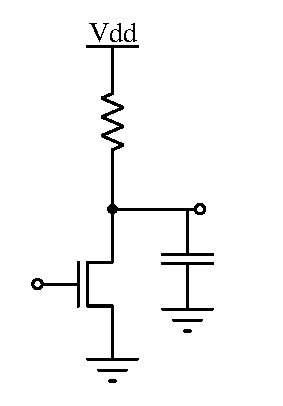
\includegraphics[scale=1]{resistive_load}\\
   % translate x=400 y=316 scale 0.38
   \putbox{0.31in}{1.70in}{1.20}{$\text{R}_\text{L}$}%
   \putbox{1.31in}{1.20in}{1.20}{out}%
   \putbox{0.06in}{0.79in}{1.20}{in}%
   \putbox{1.39in}{0.79in}{1.20}{$\text{C}_\text{L}$}%
   } % close 'parbox'
   } % close 'scalebox'
   \vspace{-\baselineskip} % this is not necessary, but looks better

			\caption{Circuit Diagram of Resistive Load Inverter}
			\label{fig::resloadckt}
		\end{center}
	\end{figure}
	
	\subsection{Netlist}
	\begin{lstlisting}
	* transistor and other circuit components definition
	m0 out in 0 0 cmosn l=2.5u w=10u
	rl supply out 7k
	cl out meas 5n
	
	* voltage source
	vdd supply 0 dc 3.3
	vin in 0 dc 3.3 pulse(0 3.3 0 0.1n 0.1n 0.5m 1m)
	vcap meas 0 dc 0
	\end{lstlisting}
	
	\subsection{Simulation Results, Analysis and Observations}
	
	Transfer characteristics were plotted for different values of $\text{R}_\text{L}$ and different W and L values for the driver NMOS. The plots obtained were as follows:
	
	\subsubsection{Variation of $\text{R}_\text{L}$}
	The curves moving to the right imply that the threshold voltage is increasing and moving to the right. Figure(\ref{fig::varying_rl_dc}) indicates that as $\text{R}_\text{L}$ increases the voltage drop across it increases. This implies that the graph moves to the left as $\text{R}_\text{L}$ increases.\\
	Figure(\ref{fig::varying_rl_time}) indicates that as $\text{R}_\text{L}$ increases the pull up resistance to the load increases. This results in the rise time increasing for an increase in $\text{R}_\text{L}$.\\
	Figure(\ref{fig::varying_rl_vcap}) indicates that as $\text{R}_\text{L}$. increases the peak current drawn by the capacitor decreases. Figure(\ref{fig::varying_rl_vdd}) indicates that the current drawn from $\text{V}_{\text{DD}}$ is the same. Table \ref{table::tablevaryrl} contains the changes in both DC and Transient parameters.
	\begin{table}[H]
		\begin{center}
			\begin{tabular}{|c|c|c|c|}
				\hline 
				\rule[-1ex]{0pt}{2.5ex} Resistance & 5k$\Omega$ & 7k$\Omega$ & 10k$\Omega$  \\ 
				\hline 
				\rule[-1ex]{0pt}{2.5ex} $\text{V}_\text{OH}$ & 3.3V & 3.3V & 3.3V \\ 
				$\text{V}_\text{OL}$ & 0.347V & 0.248V & 0.173V \\ 
				$\text{V}_\text{IL}$ & 0.661V & 0.583V & 0.528V \\ 
				$\text{V}_\text{IH}$ & 1.768V & 1.572V & 1.39V \\ 
				$\text{NM}_\text{H}$ & 1.532V & 1.728V & 1.91V \\ 
				$\text{NM}_\text{L}$ & 0.314V & 0.335V & 0.355V \\ 
				$\text{t}_\text{rise}$ & 51.83$\mu$s & 73.6$\mu$s & 0.109ms \\ 
				$\text{t}_\text{fall}$ & 10$\mu$s & 9.935$\mu$s & 9.691$\mu$s \\ 
				$\text{t}_\text{PLH}$ & 17.9$\mu$s & 24.97$\mu$s & 34.6$\mu$s \\ 
				$\text{t}_\text{PHL}$ & 4.417$\mu$s & 4.43$\mu$s & 4.455$\mu$s \\ 
				$\text{t}_\text{d}$ & 11.15$\mu$s & 14.7$\mu$s & 19.52$\mu$s \\ 
				$\text{P}_\text{avg}$ & 1.01mW  & 0.762mW & 0.561mW \\ 
				\hline 
			\end{tabular} 
		\end{center}
		\caption{Effect of varying $\text{R}_\text{L}$ on various DC and Transient Parameters}
		\label{table::tablevaryrl}
	\end{table}
	\begin{figure}[H]
		\begin{center}
			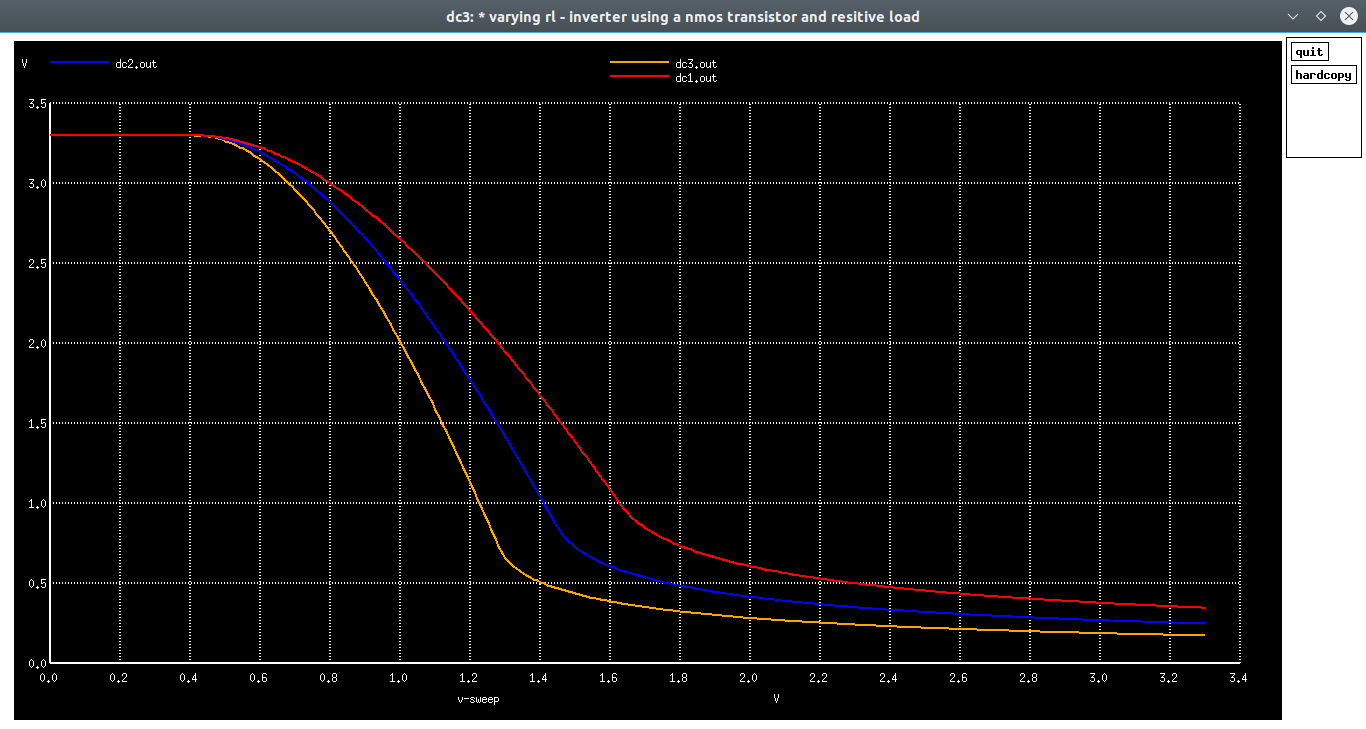
\includegraphics[scale=0.25]{images/inverter_Rl_dc.png}
			\caption{Transfer Characteristics Varying $\text{R}_\text{L}$(left to right: 10K, 7K, 5K)}
			\label{fig::varying_rl_dc}
		\end{center}
	\end{figure}
	\begin{figure}[H]
		\begin{center}
			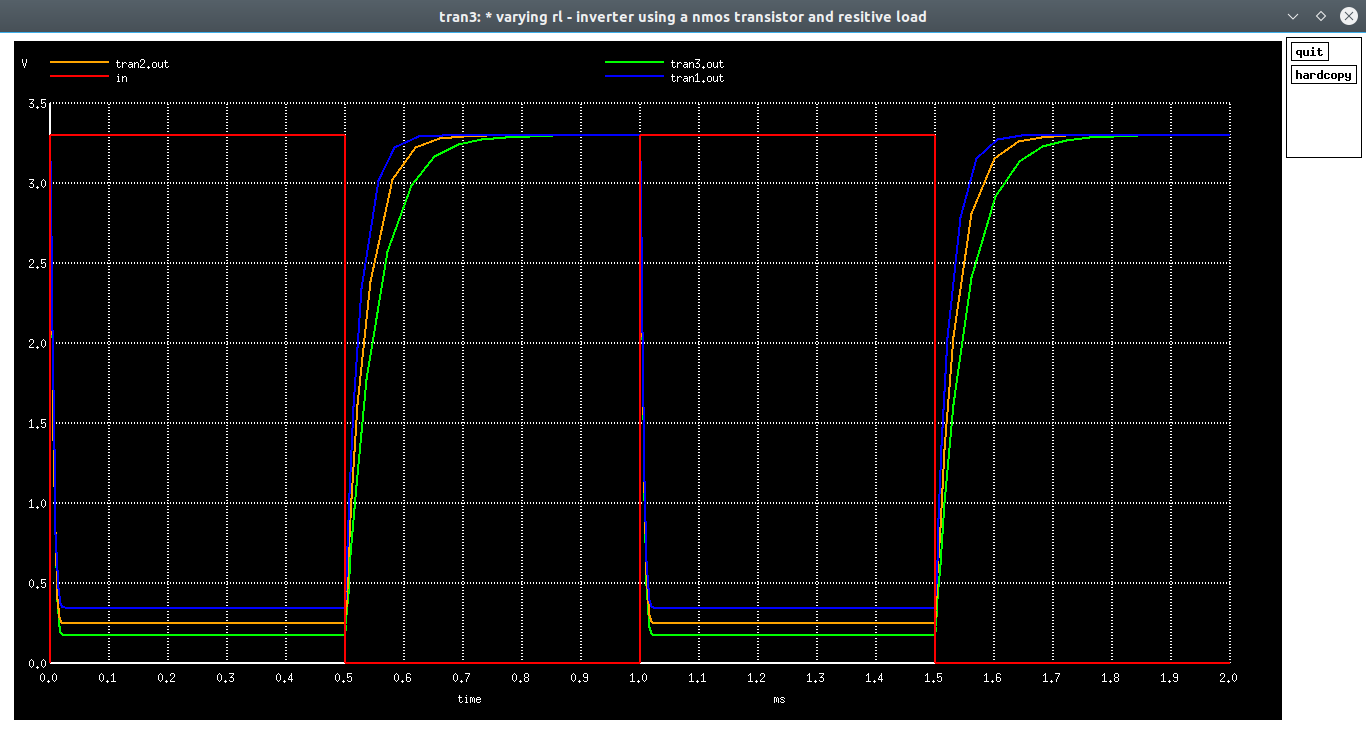
\includegraphics[scale=0.25]{images/inverter_Rl_tran.png}
			\caption{Transient Response Varying $\text{R}_\text{L}$(left to right: 5K, 7K, 10K)}
			\label{fig::varying_rl_time}
		\end{center}
	\end{figure}
	
	\begin{figure}[H]
		\begin{center}
			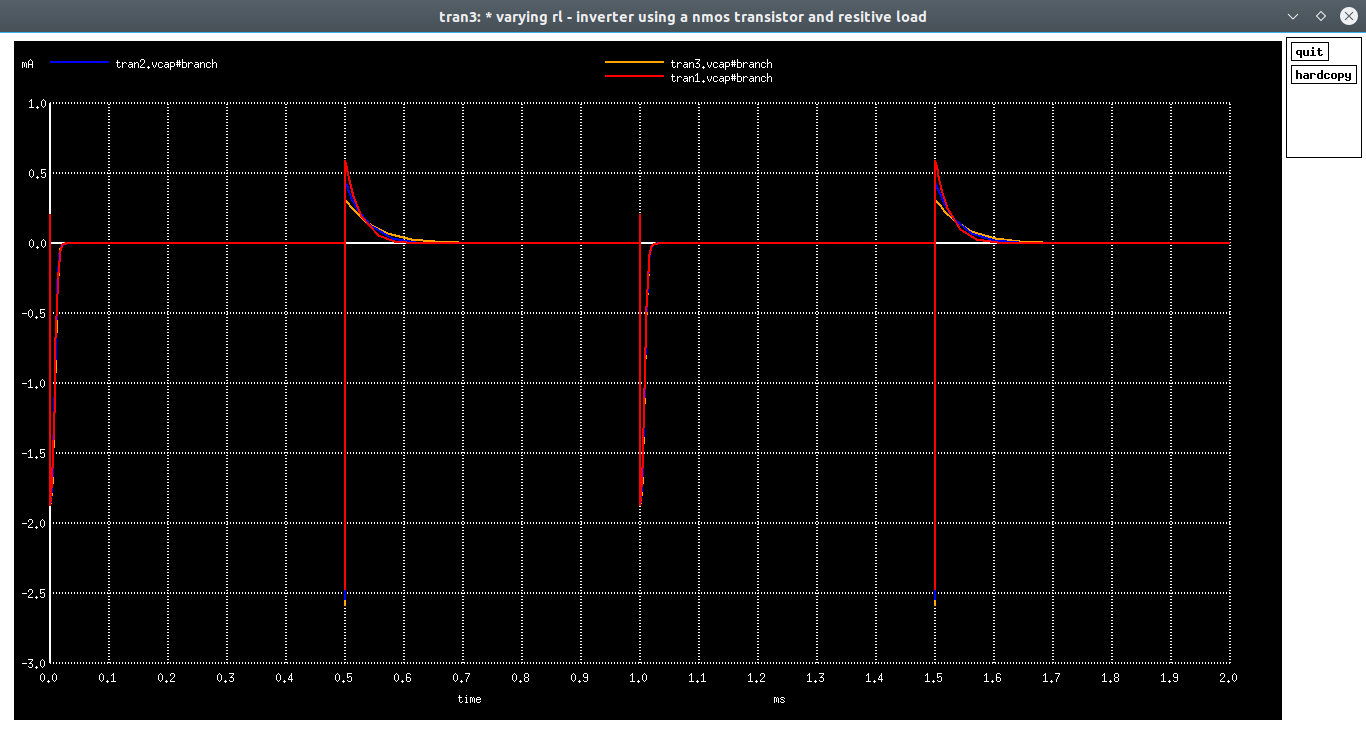
\includegraphics[scale=0.25]{images/inverter_Rl_vcap.png}
			\caption{Capacitor Current Varying $\text{R}_\text{L}$}
			\label{fig::varying_rl_vcap}
		\end{center}
	\end{figure}
	
	\begin{figure}[H]
		\begin{center}
			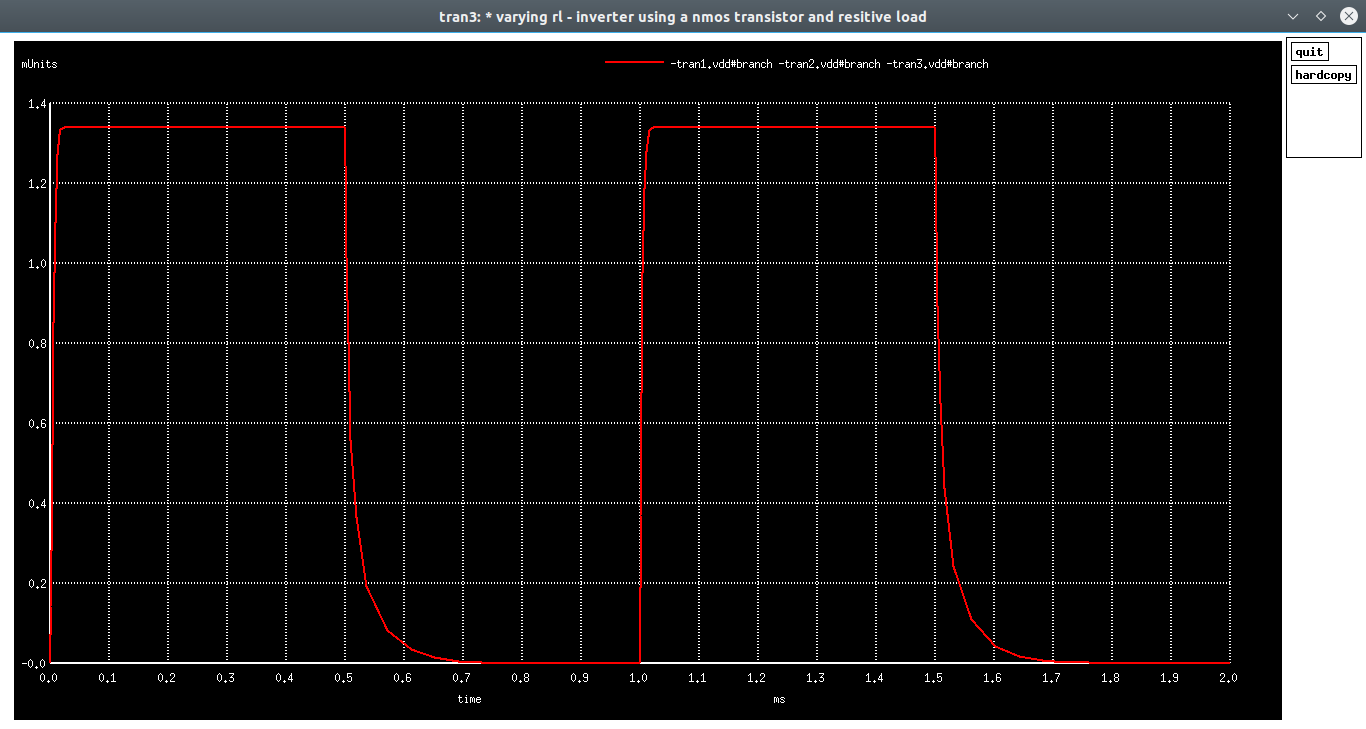
\includegraphics[scale=0.25]{images/inverter_Rl_vdd.png}
			\caption{$\text{I}_{DS}$ on Varying $\text{R}_\text{L}$}
			\label{fig::varying_rl_vdd}
		\end{center}
	\end{figure}
	
	\subsubsection{Variation of NMOS W}
	Figure(\ref{fig::varying_w_dc}) indicates that as W increases the voltage drop across the load $\text{R}_\text{L}$ increases. This implies that the graph moves to the left as W increases.\\
	Figure(\ref{fig::varying_w_time}) indicates that as W increases the pull-down resistance to the ground decreases. This results in the rise time decreaseing for an increase in W.\\
	Figure(\ref{fig::varying_w_vcap}) indicates that as W increases the peak current drawn by the capacitor increases. Figure(\ref{fig::varying_w_vdd}) indicates that the current drawn from $\text{V}_{\text{DD}}$ is the same. Table \ref{table::tablevaryw} contains the changes in both DC and Transient parameters.
	\begin{table}[H]
		\begin{center}
			\begin{tabular}{|c|c|c|c|}
				\hline 
				\rule[-1ex]{0pt}{2.5ex} W & 5$\mu$ & 10$\mu$ & 20$\mu$  \\ 
				\hline 
				\rule[-1ex]{0pt}{2.5ex} $\text{V}_\text{OH}$ & 3.3V & 3.3V & 3.3V \\ 
				$\text{V}_\text{OL}$ & 0.497V & 0.248V & 0.123V \\ 
				$\text{V}_\text{IL}$ & 0.791V & 0.58V & 0.493V \\ 
				$\text{V}_\text{IH}$ & 2V & 1.57V & 1.24V \\ 
				$\text{NM}_\text{H}$ & 1.3V & 1.73V & 2.06V \\ 
				$\text{NM}_\text{L}$ & 0.294V & 0.332V & 0.37V \\ 
				$\text{t}_\text{rise}$ & 75.21$\mu$s & 73.64$\mu$s & 72.45$\mu$s \\ 
				$\text{t}_\text{fall}$ & 20.02$\mu$s & 9.935$\mu$s & 4.82$\mu$s \\ 
				$\text{t}_\text{PLH}$ & 24.81$\mu$s & 24.97$\mu$s & 25.15$\mu$s \\ 
				$\text{t}_\text{PHL}$ & 8.56$\mu$s & 4.43$\mu$s & 2.22$\mu$s \\ 
				$\text{t}_\text{d}$ & 16.685$\mu$s & 14.4$\mu$s & 13.685$\mu$s \\ 
				$\text{P}_\text{avg}$ & 0.693mW  & 0.762mW & 0.797mW \\ 
				\hline 
			\end{tabular} 
		\end{center}
		\caption{Effect of varying W on various DC and Transient Parameters}
		\label{table::tablevaryw}
	\end{table}
	\begin{figure}[H]
		\begin{center}
			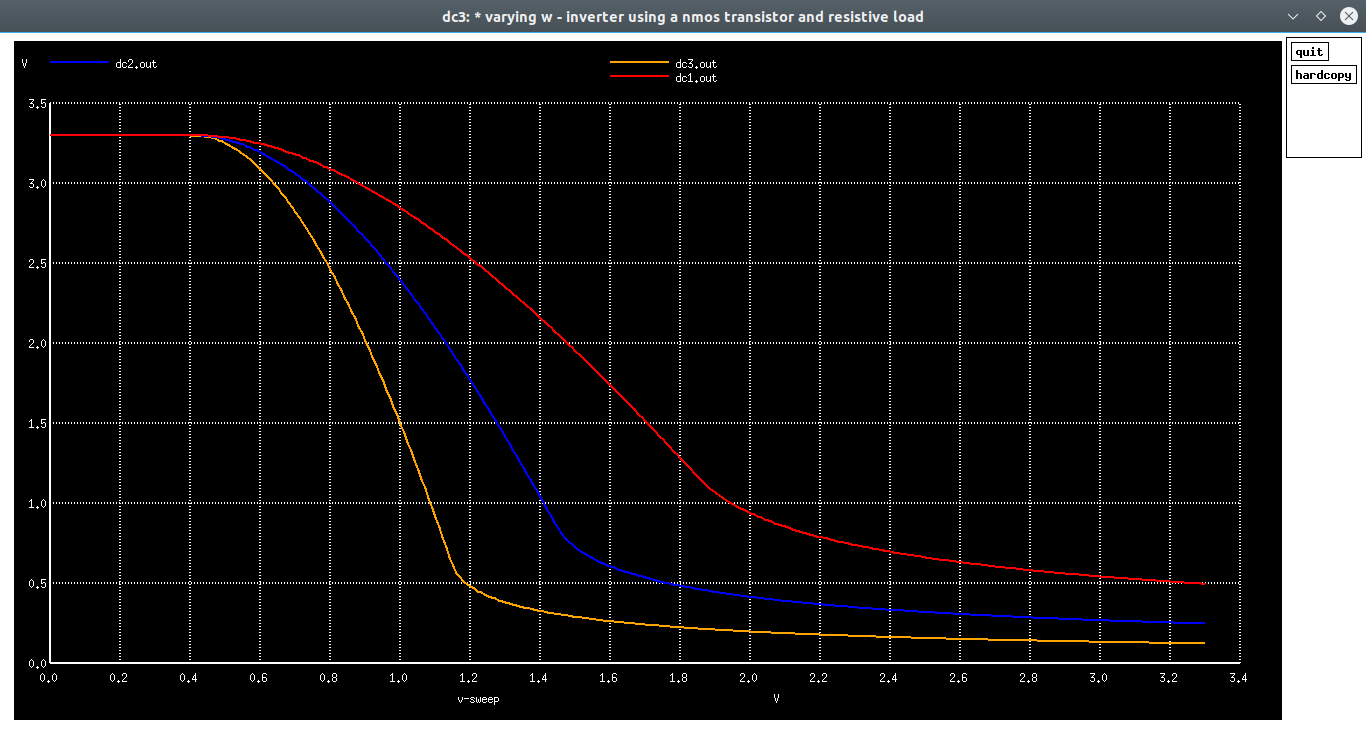
\includegraphics[scale=0.25]{images/inverter_w_dc.png}
			\caption{Transfer Characteristics Varying W}
			\label{fig::varying_w_dc}
		\end{center}
	\end{figure}
	\begin{figure}[H]
		\begin{center}
			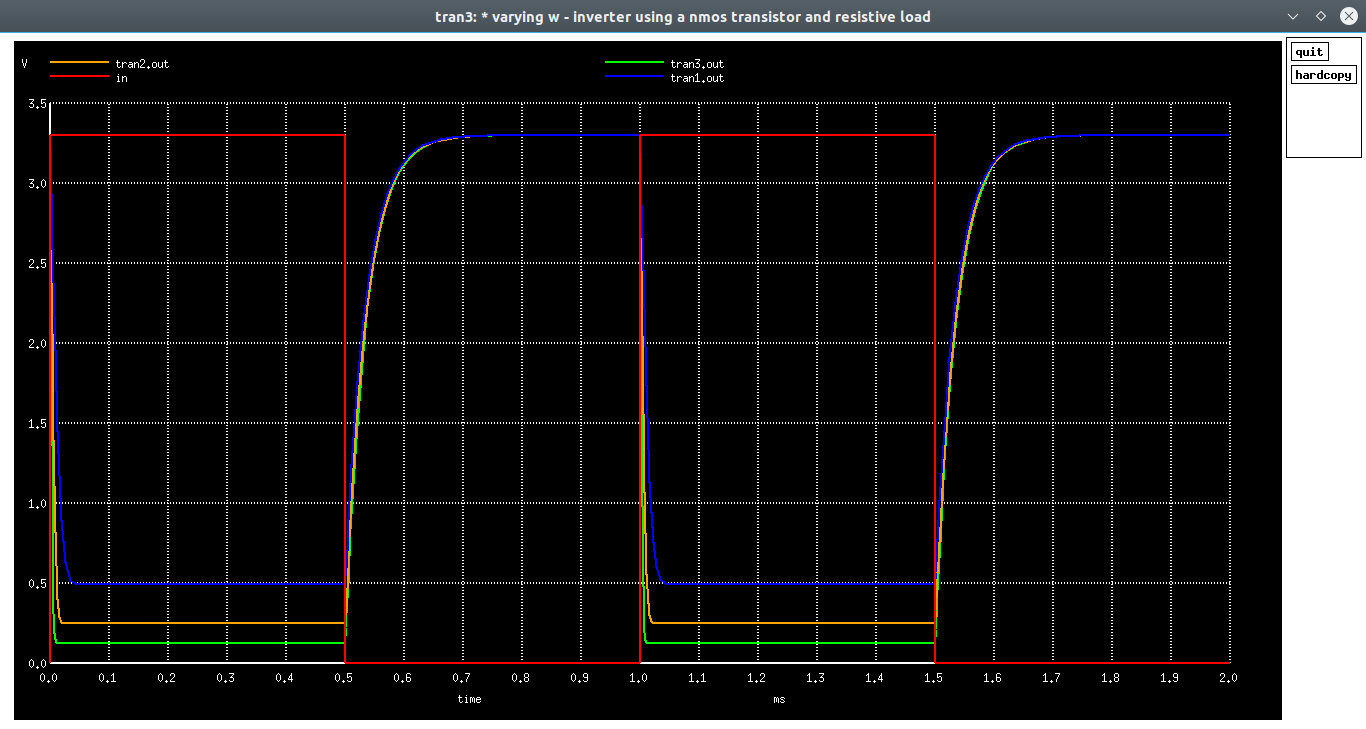
\includegraphics[scale=0.25]{images/inverter_w_tran.png}
			\caption{$\text{I}_{DS}$ on Varying W}
			\label{fig::varying_w_time}
		\end{center}
	\end{figure}
	
	\begin{figure}[H]
		\begin{center}
			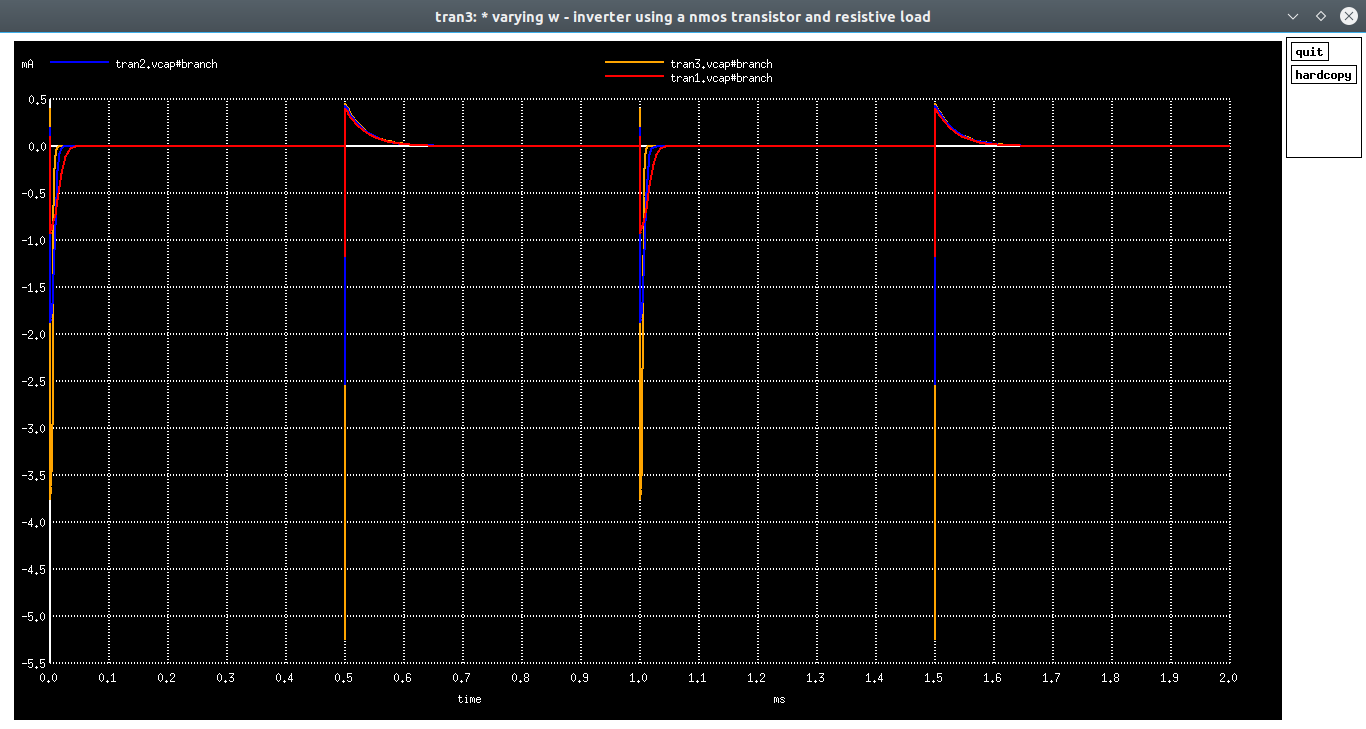
\includegraphics[scale=0.25]{images/inverter_w_vcap.png}
			\caption{Capacitor Current Varying W}
			\label{fig::varying_w_vcap}
		\end{center}
	\end{figure}
	
	\begin{figure}[H]
		\begin{center}
			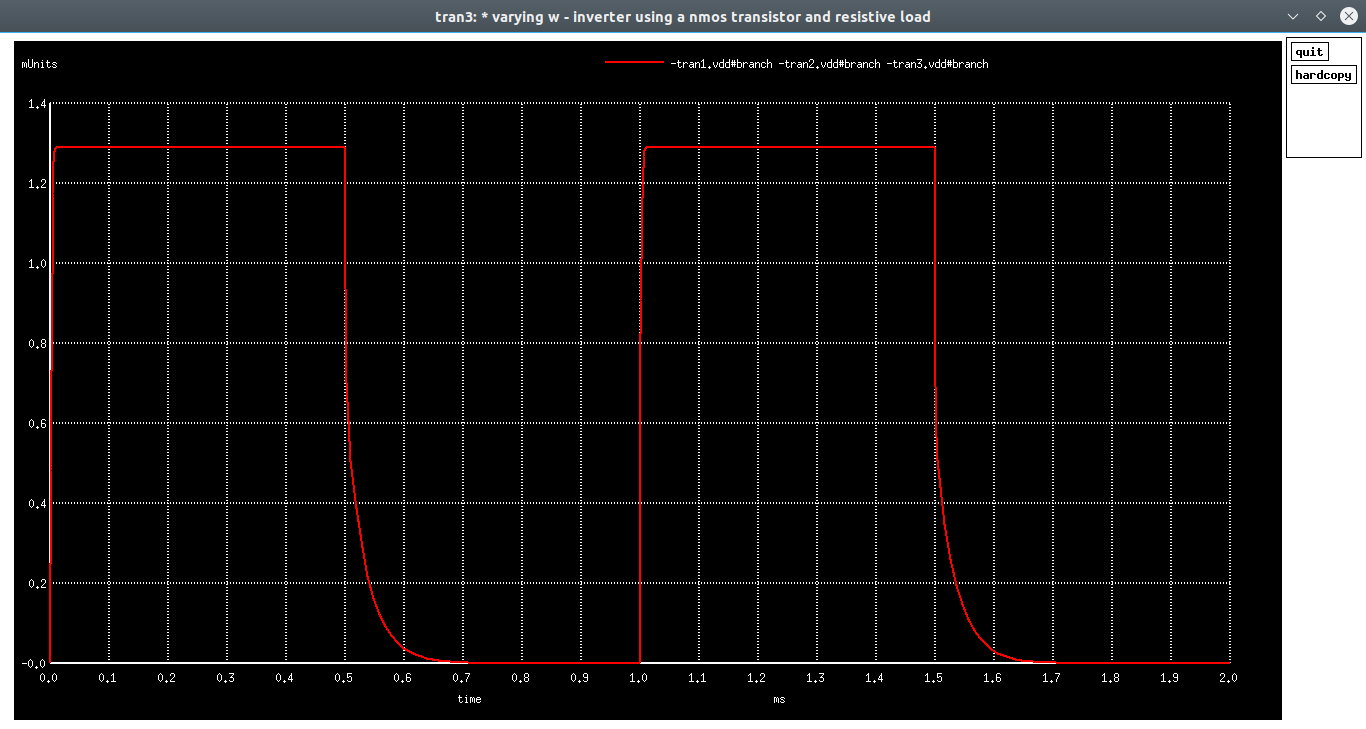
\includegraphics[scale=0.25]{images/inverter_w_vdd.png}
			\caption{Transient Response Varying W}
			\label{fig::varying_w_vdd}
		\end{center}
	\end{figure}
	
	
	
	\subsubsection{Variation of NMOS L}
	Figure(\ref{fig::varying_l_dc}) indicates that as L increases, the current decreases and the voltage drop across the load $\text{R}_\text{L}$ decreases. This implies that the graph moves to the right as L increases.\\
	Figure(\ref{fig::varying_l_time}) indicates that as L increases the pull-down resistance to the ground increases. This results in the rise time increasing for an increase in L.\\
	Figure(\ref{fig::varying_l_vdd}) indicates that the current drawn from $\text{V}_{\text{DD}}$ is the same. Table \ref{table::tablevaryl} contains the changes in both DC and Transient parameters.
	\begin{table}[H]
		\begin{center}
			\begin{tabular}{|c|c|c|c|}
				\hline 
				\rule[-1ex]{0pt}{2.5ex} L & 1$\mu$ & 2.5$\mu$ & 10$\mu$  \\ 
				\hline 
				\rule[-1ex]{0pt}{2.5ex} $\text{V}_\text{OH}$ & 3.3V & 3.3V & 3.3V \\ 
				$\text{V}_\text{OL}$ & 0.1V & 0.248V & 0.9V \\ 
				$\text{V}_\text{IL}$ & 0.455V & 0.583V & 1.24V \\ 
				$\text{V}_\text{IH}$ & 1.18V & 1.57V & 2.34V \\ 
				$\text{NM}_\text{H}$ & 2.12V & 1.73V & 0.96V \\ 
				$\text{NM}_\text{L}$ & 0.355V & 0.335V & 0.34V \\ 
				$\text{t}_\text{rise}$ & 74.31$\mu$s & 73.64$\mu$s & 78.28$\mu$s \\ 
				$\text{t}_\text{fall}$ & 4.89$\mu$s & 9.935$\mu$s & 32.62$\mu$s \\ 
				$\text{t}_\text{PLH}$ & 25.15$\mu$s & 24.97$\mu$s & 24.209$\mu$s \\ 
				$\text{t}_\text{PHL}$ & 2.32$\mu$s & 4.43$\mu$s & 12.79$\mu$s \\ 
				$\text{t}_\text{d}$ & 13.73$\mu$s & 14.7$\mu$s & 18.499$\mu$s \\ 
				$\text{P}_\text{avg}$ & 0.803mW  & 0.762mW & 0.587mW \\ 
				\hline 
			\end{tabular} 
		\end{center}
		\caption{Effect of varying L on various DC and Transient Parameters}
		\label{table::tablevaryl}
	\end{table}
	\begin{figure}[H]
		\begin{center}
			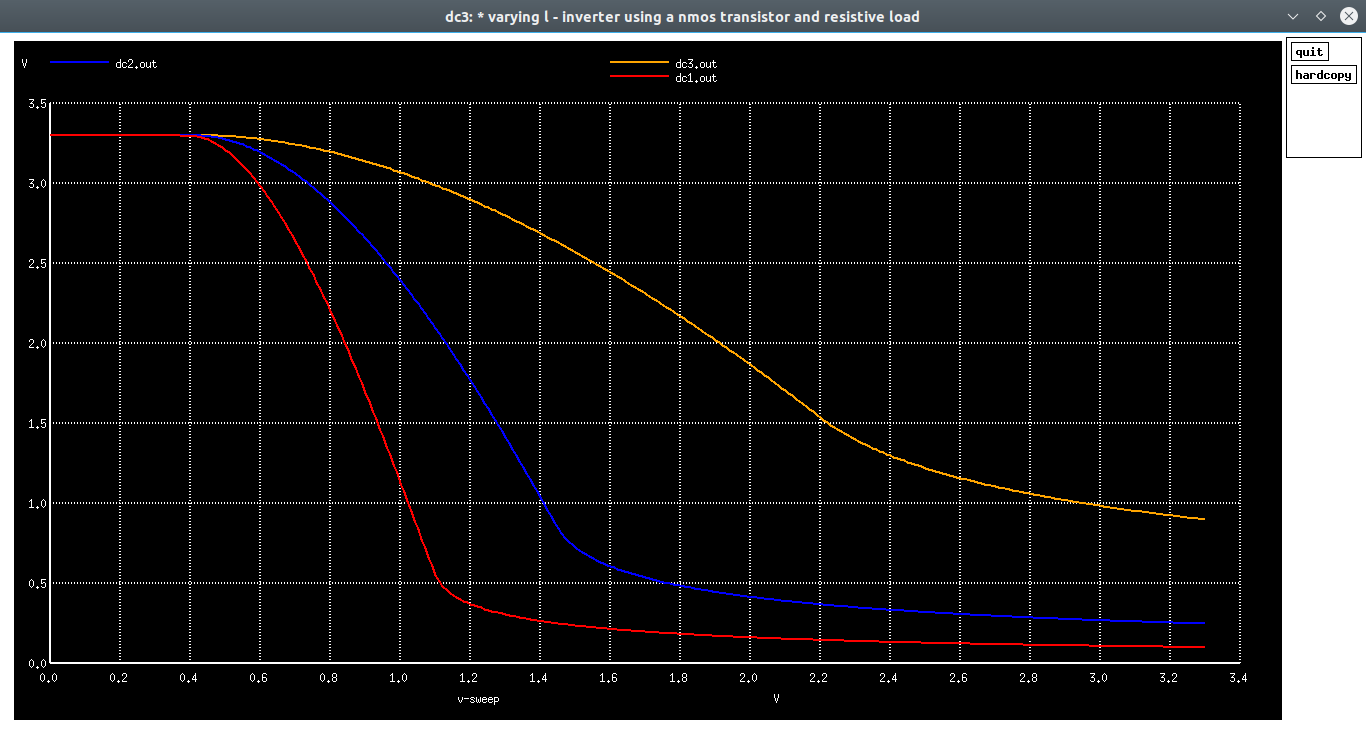
\includegraphics[scale=0.25]{images/inverter_l_dc.png}
			\caption{Transfer Characteristics Varying L}
			\label{fig::varying_l_dc}
		\end{center}
	\end{figure}
	\begin{figure}[H]
		\begin{center}
			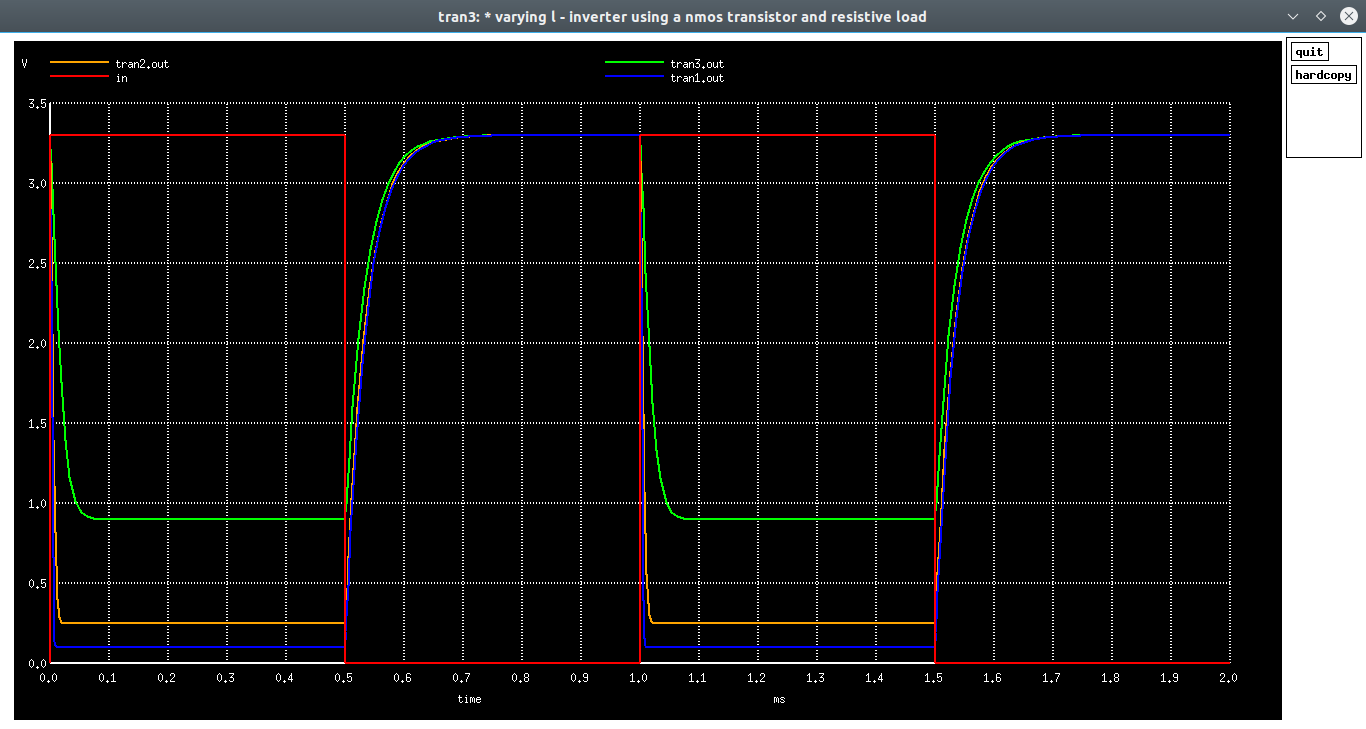
\includegraphics[scale=0.25]{images/inverter_l_tran.png}
			\caption{Transient Response Varying L}
			\label{fig::varying_l_time}
		\end{center}
	\end{figure}
	
	\begin{figure}[H]
		\begin{center}
			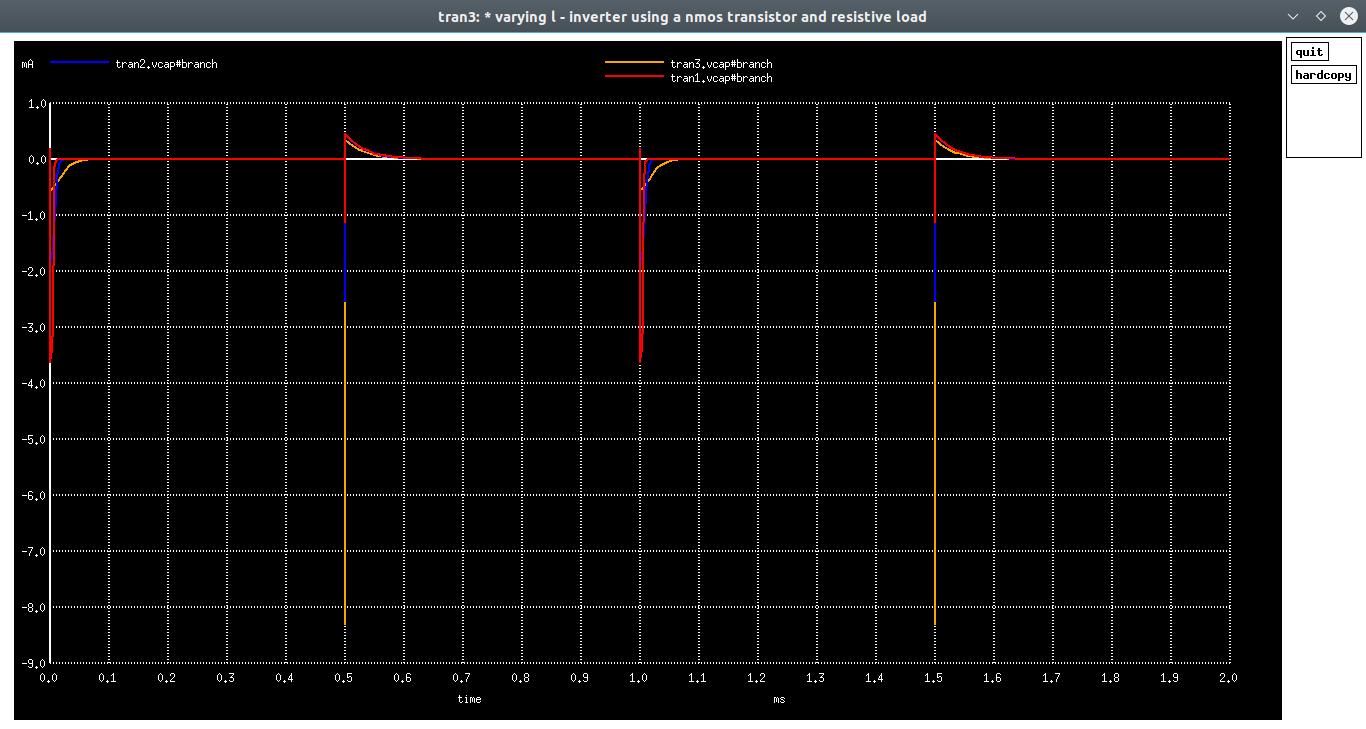
\includegraphics[scale=0.25]{images/inverter_l_vcap.png}
			\caption{Capacitor Current Varying L}
			\label{fig::varying_l_vcap}
		\end{center}
	\end{figure}
	\begin{figure}[H]
		\begin{center}
			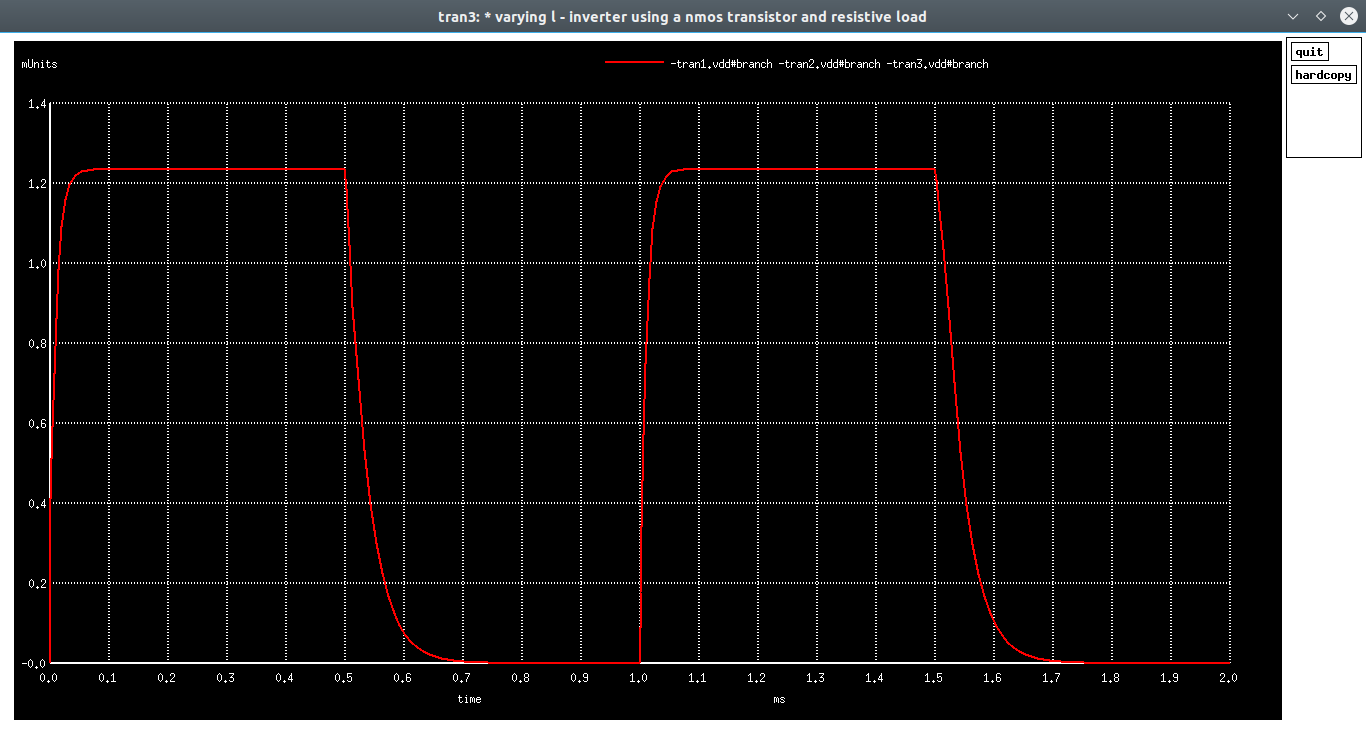
\includegraphics[scale=0.25]{images/inverter_l_vdd.png}
			\caption{$\text{I}_{DS}$ on Varying L}
			\label{fig::varying_l_vdd}
		\end{center}
	\end{figure}
	
	\subsubsection{Variation of $\text{C}_\text{L}$}
	On varying $\text{C}_\text{L}$, no variation in DC parameters($\text{NM}_\text{H}$, $\text{NM}_\text{L}$) is observed, as they are independent of the load capacitance. Whereas for transient parameters, we observe that as $\text{C}_\text{L}$ increases, the rise time and fall time increase, as a larger value of capacitance takes more time to charge and discharge. Table \ref{table::tablevarcl} contains the changes in both DC and Transient parameters.
	\begin{table}[H]
		\begin{center}
			\begin{tabular}{|c|c|c|}
				\hline 
				\rule[-1ex]{0pt}{2.5ex} $\text{C}_\text{L}$ & 0.1nF & 20nF\\ 
				\hline 
				\rule[-1ex]{0pt}{2.5ex} 
				$\text{V}_\text{OH}$ & 3.3V & 3.3V  \\ 
				$\text{V}_\text{OL}$ & 0.2481V & 0.2481V \\ 
				$\text{V}_\text{IL}$ & 0.583V & 0.583V \\ 
				$\text{V}_\text{IH}$ & 1.57V & 1.572V \\ 
				$\text{NM}_\text{H}$ & 1.728V & 1.728V\\ 
				$\text{NM}_\text{L}$ & 0.3349V & 0.3349V \\ 
				$\text{t}_\text{rise}$ & 1.55$\mu$s & 0.302ms\\ 
				$\text{t}_\text{fall}$ & 0.193$\mu$s & 39.86$\mu$s\\ 
				$\text{t}_\text{PLH}$ & 0.501$\mu$s & 99.77$\mu$s\\ 
				$\text{t}_\text{PHL}$ & 87.72ns & 18.08$\mu$s\\ 
				$\text{t}_\text{d}$ & 0.294$\mu$s & 58.85$\mu$s\\ 
				$\text{P}_\text{avg}$ & 0.702mW  & 0.8862mW\\ 
				\hline 
			\end{tabular} 
		\end{center}
		\caption{Effect of varying $\text{C}_\text{L}$ on various DC and Transient Parameters}
		\label{table::tablevarcl}
	\end{table}
	\begin{figure}[H]
		\begin{center}
			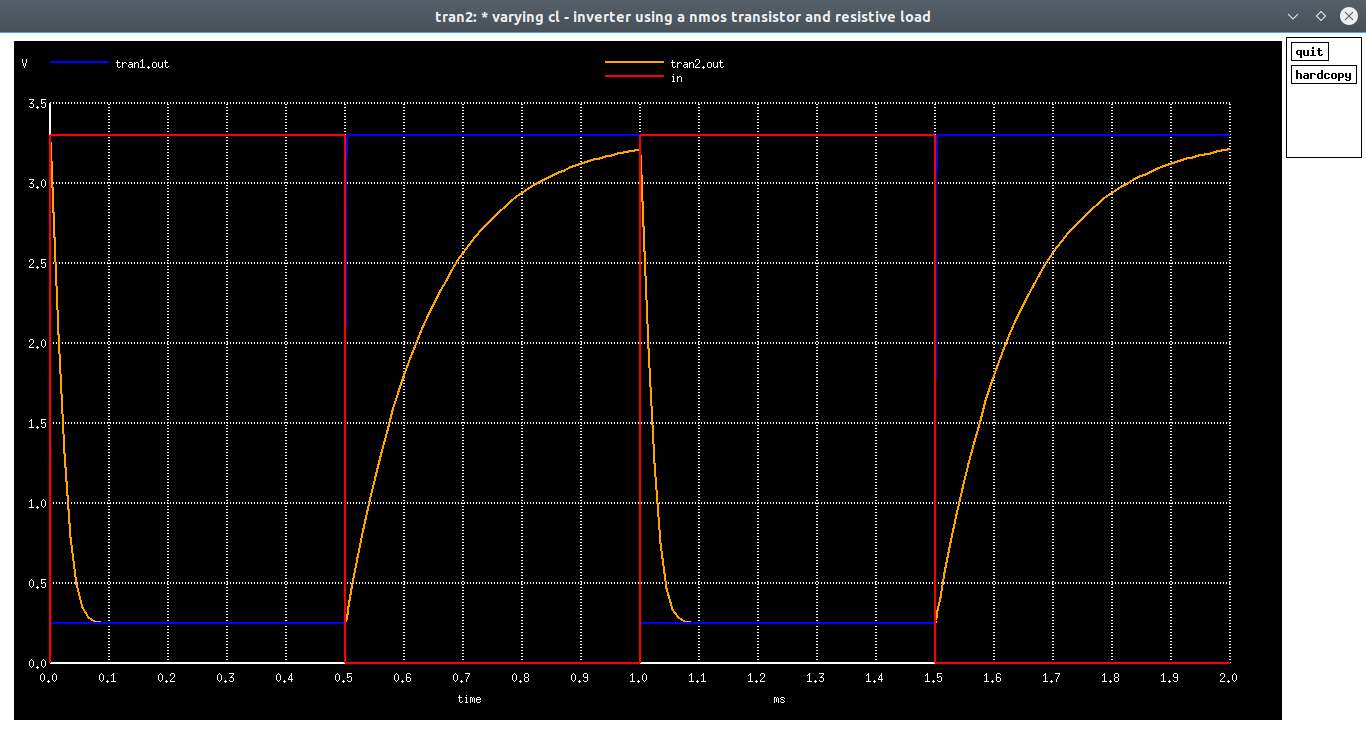
\includegraphics[scale=0.25]{images/inverter_cl_tran.png}
			\caption{Transient Response Varying $\text{C}_\text{L}$}
			\label{fig::varying_cl_tran}
		\end{center}
	\end{figure}
	
	\begin{figure}[H]
		\begin{center}
			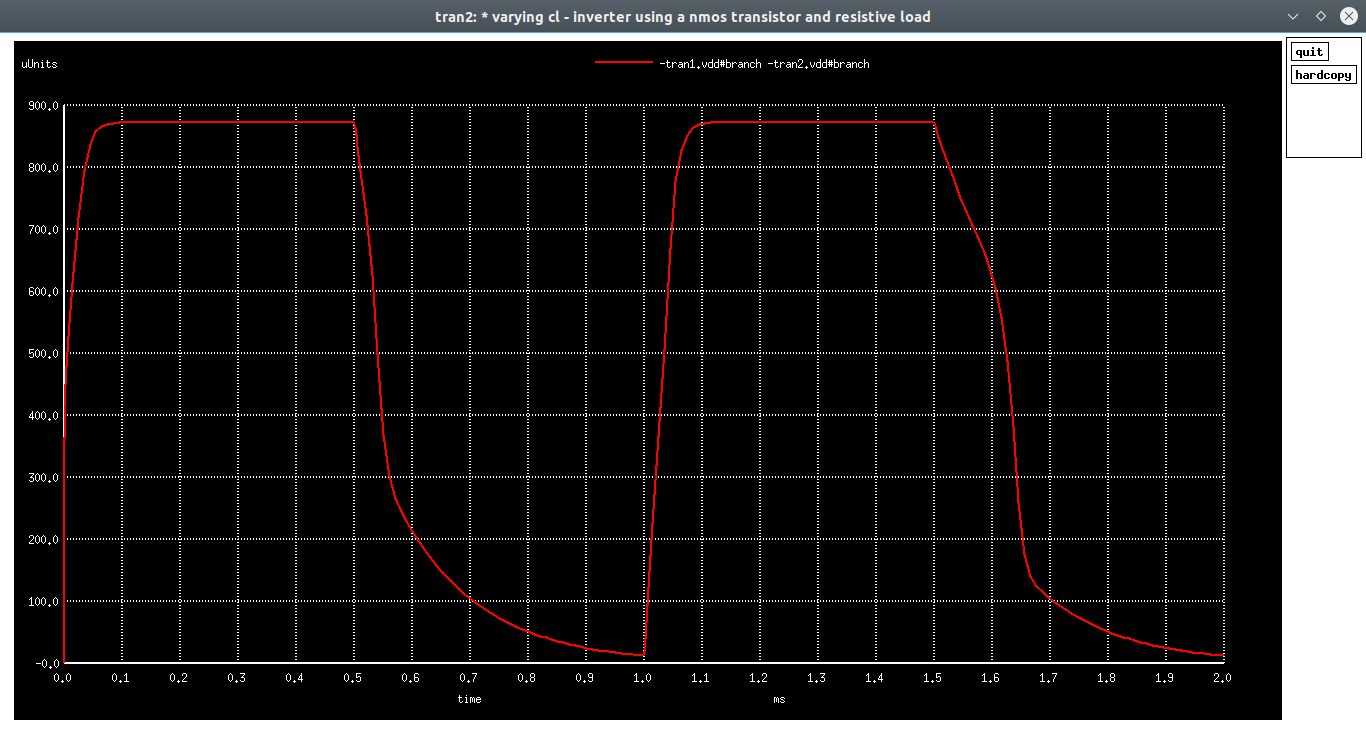
\includegraphics[scale=0.25]{images/inverter_cl_vdd.png}
			\caption{$\text{I}_{DS}$ on Varying $\text{C}_\text{L}$}
			\label{fig::varying_cl_vdd}
		\end{center}
	\end{figure}
	\begin{figure}[H]
		\begin{center}
			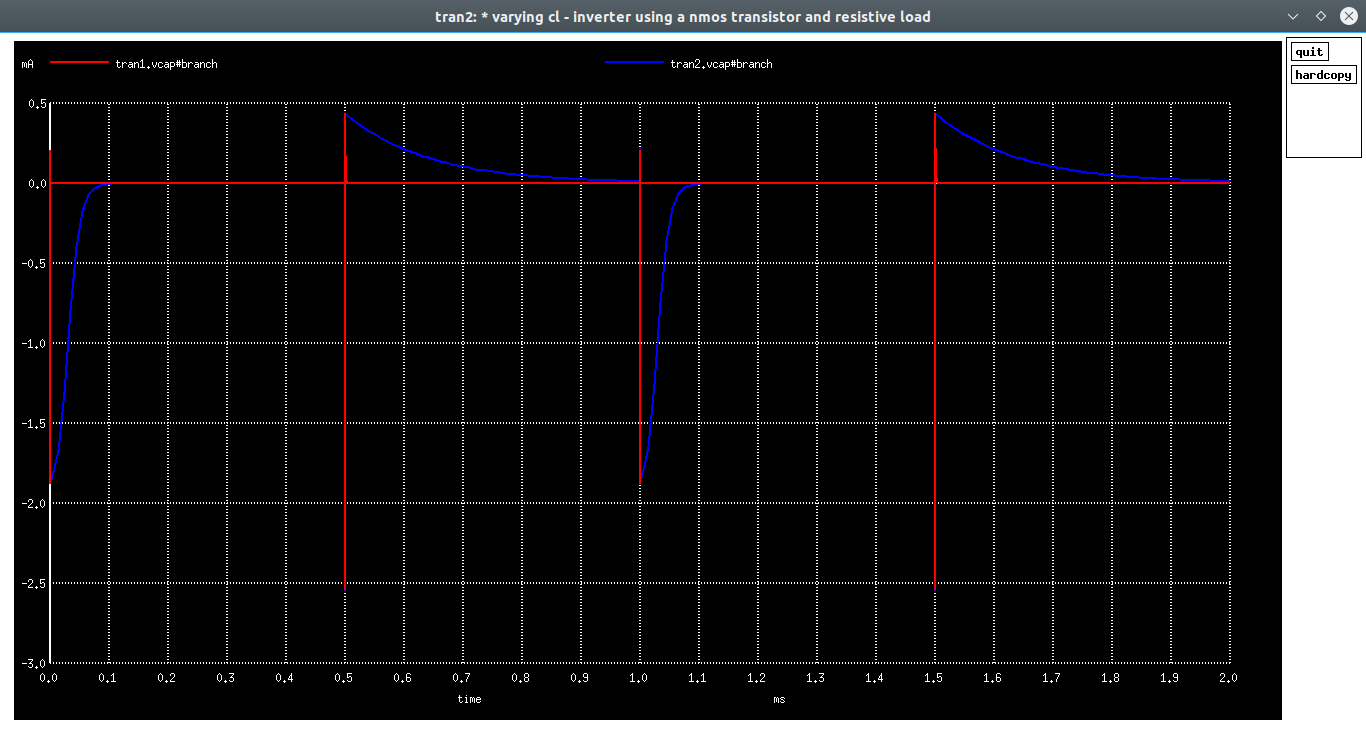
\includegraphics[scale=0.25]{images/inverter_cl_vcap.png}
			\caption{Capacitor current on Varying $\text{C}_\text{L}$}
			\label{fig::varying_cl_vcap}
		\end{center}
	\end{figure}
	
	\subsection{Conclusion}
	The experiment was performed, and all parameters were extracted and analysed. The values obtained agreed with theory, and hence simulations were verified. NGSPICE was the simulator used for this task.
	
	
	
	
	\newpage
	\section{CMOS Inverter Layout and Characterisation} 
	\rhead{CMOS Inverter Layout and Characterisation}
	\subsection{Aim}
	To learn layout, extract, LVS and characterization processes in the design flow with CMOS inverter as example, and to compute parametrs such as input capactiance, output capacitance, rise time and fall time for various loads.
	\subsection{Circuit Diagram}
	\begin{figure}[H]
		\begin{center}
			% XCircuit output "cmos_inverter.tex" for LaTeX input from cmos_inverter.eps
\def\putbox#1#2#3#4{\makebox[0in][l]{\makebox[#1][l]{}\raisebox{\baselineskip}[0in][0in]{\raisebox{#2}[0in][0in]{\scalebox{#3}{#4}}}}}
\def\rightbox#1{\makebox[0in][r]{#1}}
\def\centbox#1{\makebox[0in]{#1}}
\def\topbox#1{\raisebox{-0.60\baselineskip}[0in][0in]{#1}}
\def\midbox#1{\raisebox{-0.20\baselineskip}[0in][0in]{#1}}
   \scalebox{1}{
   \normalsize
   \parbox{1.64583in}{
   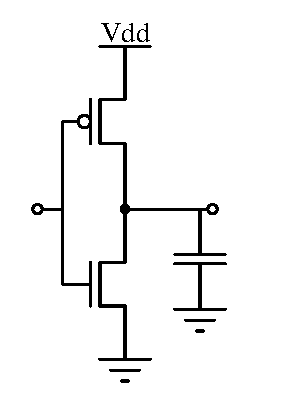
\includegraphics[scale=1]{cmos_inverter}\\
   % translate x=416 y=316 scale 0.38
   \putbox{1.39in}{1.20in}{1.20}{out}%
   \putbox{0.06in}{1.29in}{1.20}{in}%
   \putbox{1.47in}{0.79in}{1.20}{$\text{C}_\text{L}$}%
   } % close 'parbox'
   } % close 'scalebox'
   \vspace{-\baselineskip} % this is not necessary, but looks better

			\caption{Circuit Diagram of CMOS Inverter}
			\label{fig::cmosinvckt}
		\end{center}
	\end{figure}
	
	\subsection{Introduction}
	Inverter is one that inverts the signal supplied at its input. If input is made high or logic level is 1, then the output has a logic level 0 and vice-versa. CMOS stands for Complementary Metal Oxide Semiconductor. CMOS is one of the various families in logic gate design in Digital VLSI. A major difference in this family is, there is both a pull-up network as well as the pull-down network and only one of the path is on at any given time. The output is taken at the junction of pull-up and pull-down network. When pull-up network constructed using PMOS is ON, output capacitor is charged by the supply and when pull-down network constructed using NMOS is ON, the capacitor initially charged now discharges through this path to ground.
	
	\subsection{Layout}
	\begin{figure}[H]
		\begin{center}
			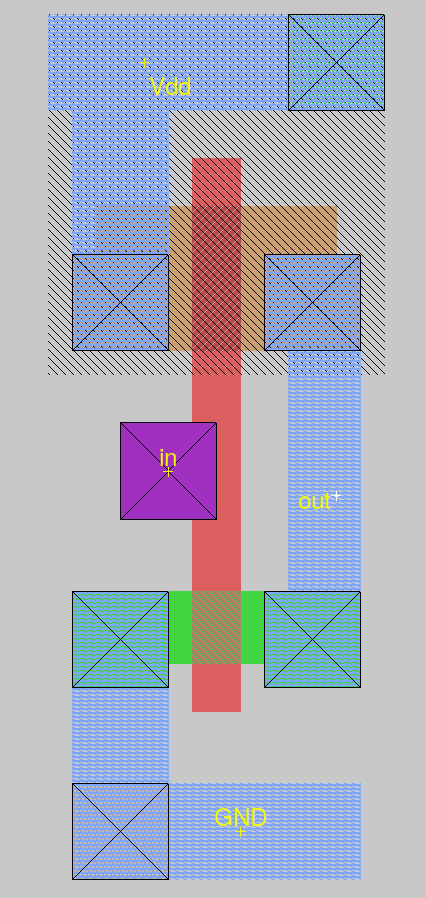
\includegraphics[scale = 0.5]{images/layout.png}
			\caption{Layout of CMOS Inverter}
			\label{fig::cmoslayout}
		\end{center}
	\end{figure}
	
	From the layout in Figure(\ref{fig::cmoslayout}), it is seen that the width of the pdiffusion layer is twice the ndiffusion layer. This is to compensate for the mobility of holes compared to electrons, so as to make the $\text{t}_\text{rise} \approx \text{t}_\text{fall}$.
	\subsection{Expected Netlist}
	\begin{lstlisting}
	m0 out in 0 0 cmosn l=0.25u w=10u
	m1 out in Vdd Vdd cmosp l=0.25u w=31u
	cl out 0 5n
	\end{lstlisting}
	\subsection{Netlist extracted from Magic}
	\begin{lstlisting}
	M1000 out in Vdd Vdd cmosp w=6 l=2
	+  ad=28 pd=22 as=28 ps=22
	M1001 out in Gnd Gnd cmosn w=3 l=2
	+  ad=19 pd=18 as=19 ps=18
	C0 in Gnd 4.0fF
	C1 out Gnd 2.07fF
	\end{lstlisting}
	
	\subsection{Analysis and Observation}
	Area of the inverter cell = 504 microns 
	\par Input capacitance = 4 fF
	\par Output capacitance = 2.07 fF
	\par Sum of all nodal capacitance = 0.02540 pF
	
	The DC transfer characteristics is shown in Figure(\ref{fig::layout_dc}). It is seen that the transfer characteristics does not change  with different load capacitance $\text{C}_\text{L}$ 
	\begin{figure}[H]
		\begin{center}
			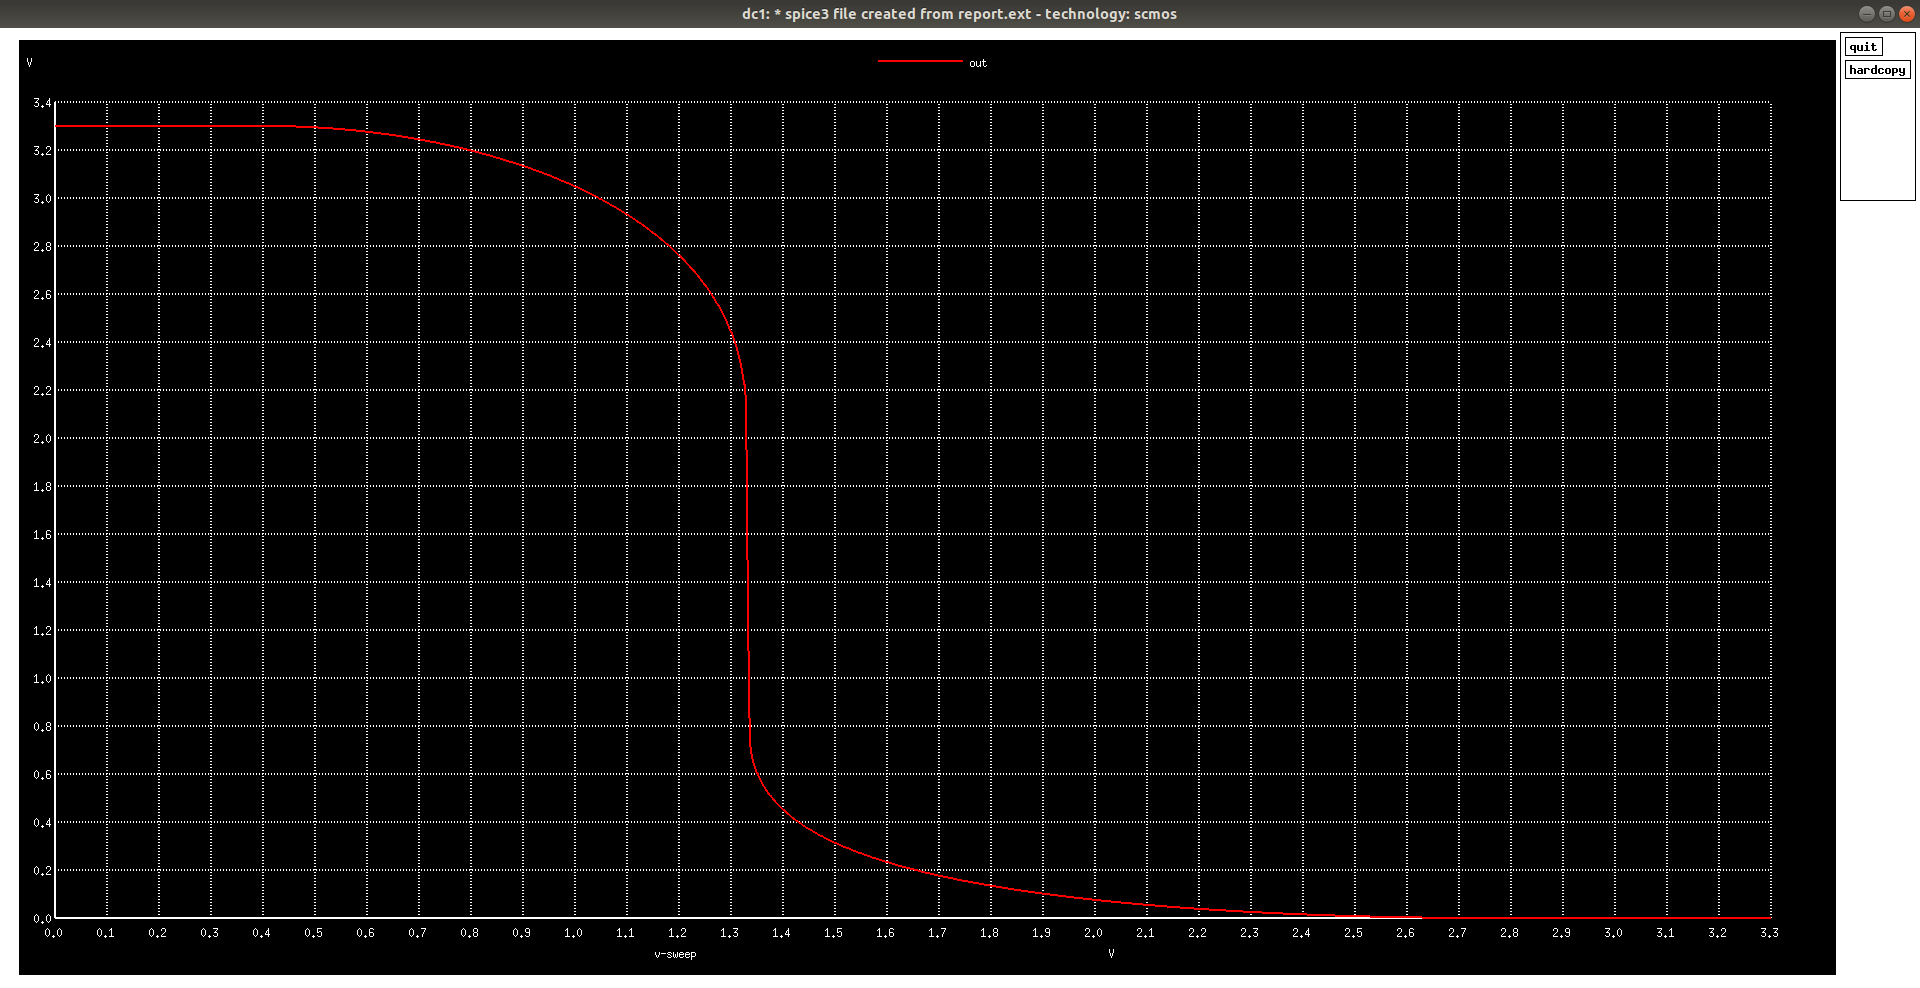
\includegraphics[scale = 0.18]{images/layout_dc.png}
			\caption{CMOS Inverter transfer characteristics}
			\label{fig::layout_dc}
		\end{center}
	\end{figure}
	
	The transient response of the CMOS inverter can be seen in Figure(\ref{fig::layout_tran}). It can be seen that as the lthe load capacitance $\text{C}_\text{L}$ increases, the output takes time to reach the maximum voltage. This is further supported by the values in Table(\ref{table::tablevarycllayout}). The rise and the tfall increases for increase in the load capacitance.\\
	
	The value of the trise and the tfall can be approximated to 
	\begin{align}
	t_{rise} = 2.2*R_{p_{eff}}*C \\ 
	t_{fall} = 2.2*R_{n_{eff}}*C 
	\end{align}
	where $R_{p_{eff}}$ and $R_{n_{eff}}$ are the effective resistances exhibited by the PMOS and the NMOS during the pull-up and the pull-down phase respectively. 
	\begin{figure}[H]
		\begin{center}
			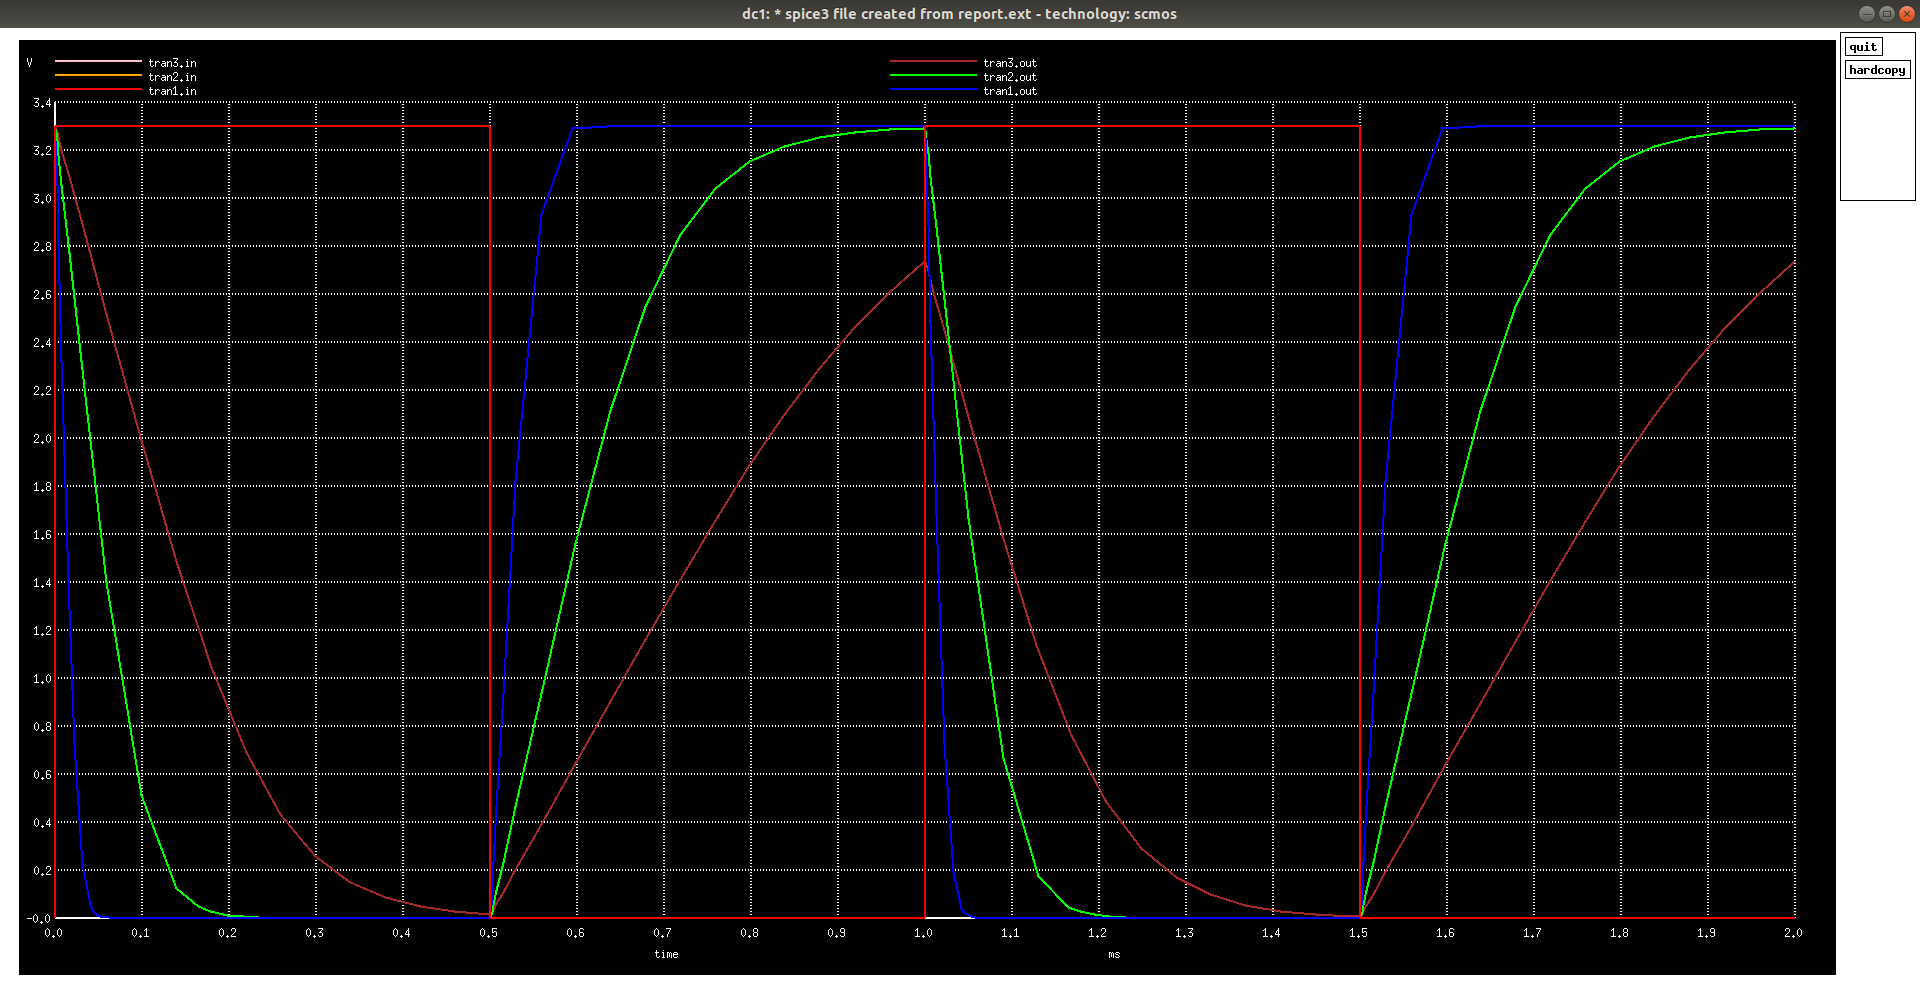
\includegraphics[scale = 0.2]{images/layout_tran_cl.png}
			\caption{CMOS Inverter transient characteristics with various $\text{C}_\text{L}$(5nF, 20nF, 50nF)}
			\label{fig::layout_tran}
		\end{center}
	\end{figure}
	\begin{table}[H]
		\begin{center}
			\begin{tabular}{|c|c|c|c|}
				\hline 
				\rule[-1ex]{0pt}{2.5ex} $\text{C}_\text{L}$ & 5nF & 20nF & 50nF \\ 
				\hline 
				\rule[-1ex]{0pt}{2.5ex}
				$\text{t}_\text{rise}$ & 56.61$\mu$s & 0.223ms & - \\ 
				$\text{t}_\text{fall}$ & 26.64$\mu$s & 0.107ms & 0.25805ms \\ 
				$\text{t}_\text{PLH}$ & 26.3$\mu$s & 0.1045ms & 0.2568ms \\ 
				$\text{t}_\text{PHL}$ & 12.77$\mu$s & 0.0109ms & 0.1262ms \\ 
				$\text{t}_\text{d}$ & 19.55$\mu$s & 0.07781ms & 0.191ms \\ 
				$\text{P}_\text{avg}$ & 54.45$\mu$W  & 0.2173mW & 0.449mW \\ 
				$\text{P}_\text{dynamic}$ & 0.111mW  & 0.435mW & 0.946mW \\ 
				\hline $\text{V}_\text{OH}$ &\multicolumn{3}{|c|}{3.3V}\\ 
				$\text{V}_\text{OL}$ & \multicolumn{3}{|c|}{4.83nV} \\ 
				$\text{V}_\text{IL}$ & \multicolumn{3}{|c|}{1.0034V} \\ 
				$\text{V}_\text{IH}$ & \multicolumn{3}{|c|}{1.4996V} \\ 
				$\text{NM}_\text{H}$ & \multicolumn{3}{|c|}{1.8003V} \\ 
				$\text{NM}_\text{L}$ & \multicolumn{3}{|c|}{1.0034V}\\ 
				\hline 
			\end{tabular} 
		\end{center}
		\caption{Effect of varying $\text{C}_\text{L}$ on various DC and Transient Parameters}
		\label{table::tablevarycllayout}
	\end{table}
	
	\subsection{Conclusion}
	The experiment was performed, and a layout for CMOS inverter was designed using MAGIC software. The netlist was extracted and compared with a netlist designed for CMOS inverter, and was found to be the same. Various parameters have been found out and analysed.
	
\end{document}